\documentclass[a4paper,11pt]{article}
%\usepackage{tabular}
\usepackage[dvipdfm]{graphicx}
\usepackage[dvipdfm]{color}
\usepackage{wrapfig}
\usepackage{amsmath, amssymb}
\usepackage{txfonts}
\usepackage{multirow}
\usepackage{subfigure}
\usepackage{ulem}
\usepackage{graphicx}
\usepackage{lscape}

\setlength{\textwidth}{150mm}  
\setlength{\textheight}{232mm}

\setlength{\oddsidemargin}{-2mm}
\setlength{\evensidemargin}{-2mm}
\setlength{\topmargin}{-15mm}
%%%%%%%%%%%%%%%%%%%%%%%%%%%%%%%%%%%%%%%%%%%%%%%%%%%%%%%%%%%%%%%
\begin{document}


\pagestyle{empty}

\begin{rightline}
{Jan-23-2014 Ver.2}
\end{rightline}


\noindent
\textbf{Plotting all events (386 events, 320 runs). Data is accurate to a minute.}\\

\noindent
Some event times were fixed for 2010 (Ver.2).\\
$\ast$ X axis tick-marks are located on Mondays.

\begin{figure}[htbp]
\begin{center}
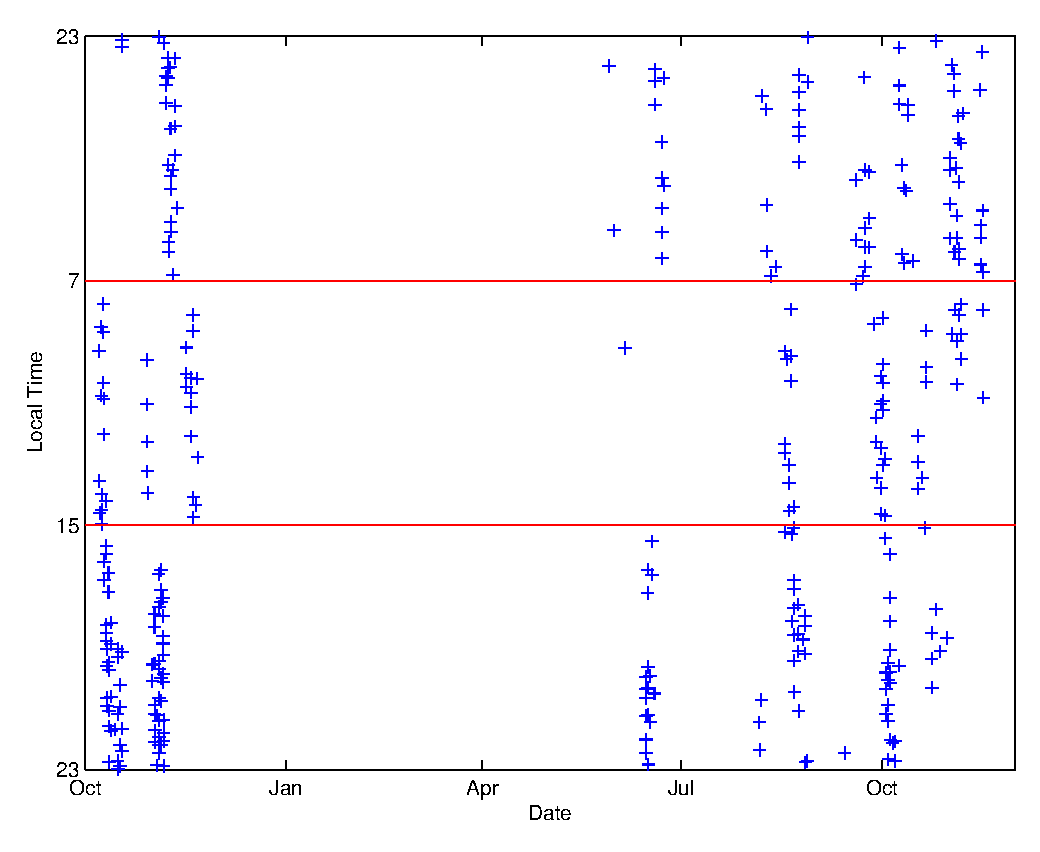
\includegraphics[width =10cm]{PlotTime.eps}
\caption{Events(runs) day time distribution - 2010\&2011}
\end{center}
\label{twoyears}
\end{figure}

\begin{figure}[htbp]
\begin{center}
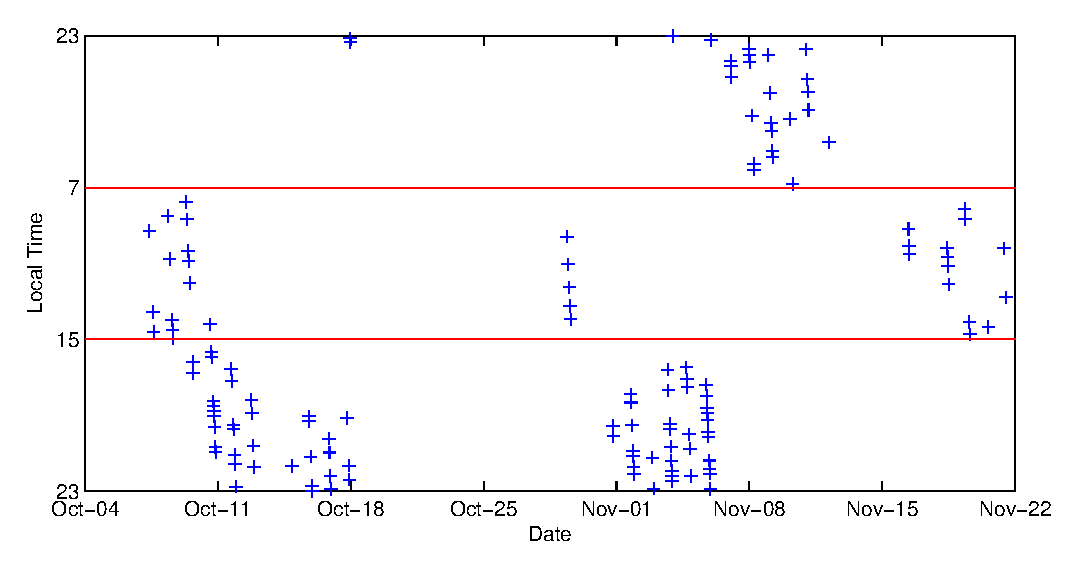
\includegraphics[width =11cm]{PlotTime2010.eps}
\caption{Events(runs) clock time distribution - 2010}
\end{center}
\label{2010}
\end{figure}

\begin{figure}[htbp]
\begin{minipage}{1.0\hsize}
\begin{center}
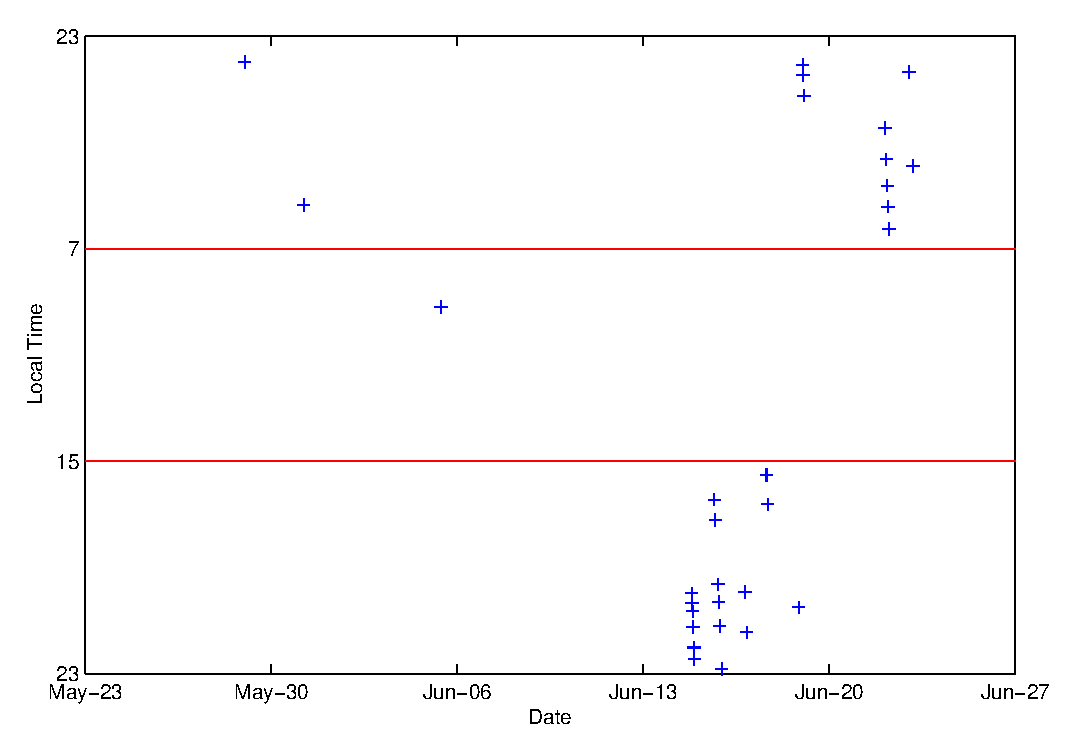
\includegraphics[width =8cm]{PlotTime2011_1.eps}
\\
\end{center}
\end{minipage}
\begin{minipage}{1.0\hsize}
\begin{center}
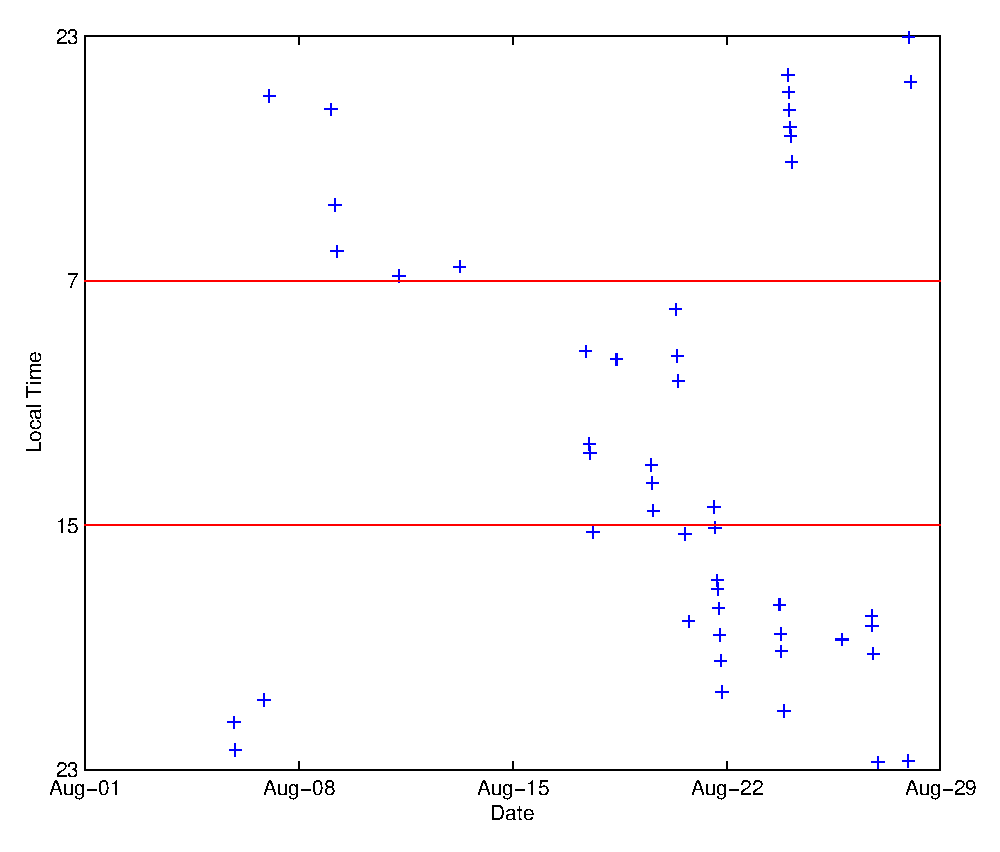
\includegraphics[width =8cm]{PlotTime2011_2.eps}
\\
\end{center}
\end{minipage}
\begin{minipage}{1.0\hsize}
\begin{center}
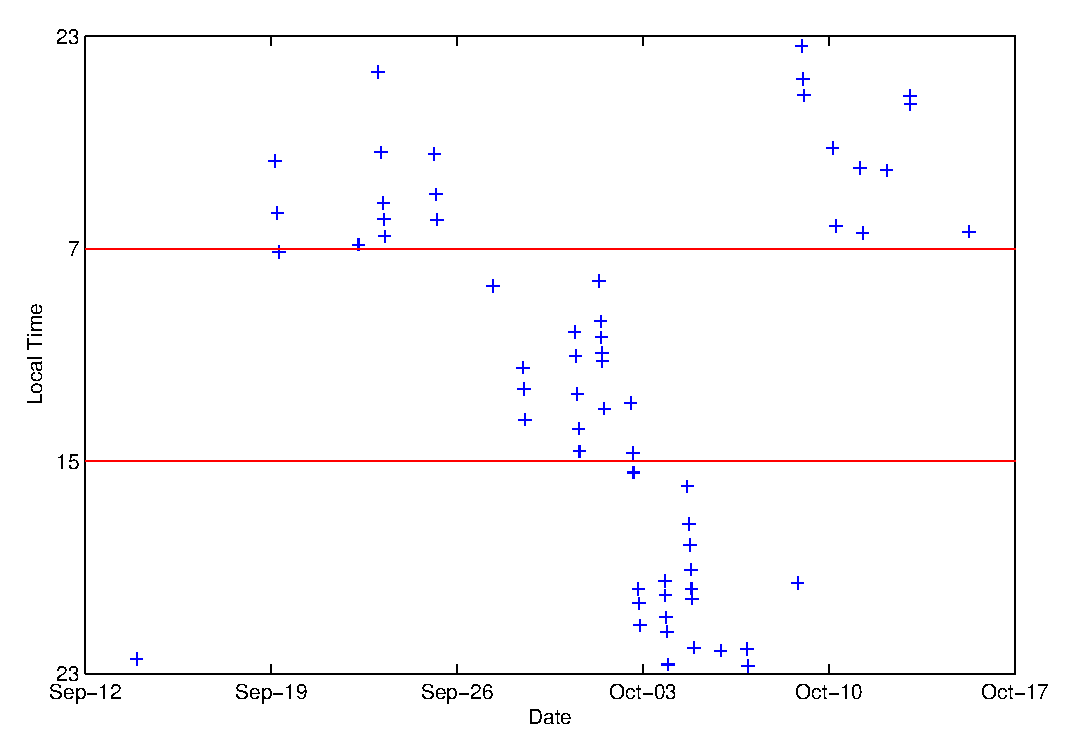
\includegraphics[width =8cm]{PlotTime2011_3.eps}
\\
\end{center}
\end{minipage}
\begin{minipage}{1.0\hsize}
\begin{center}
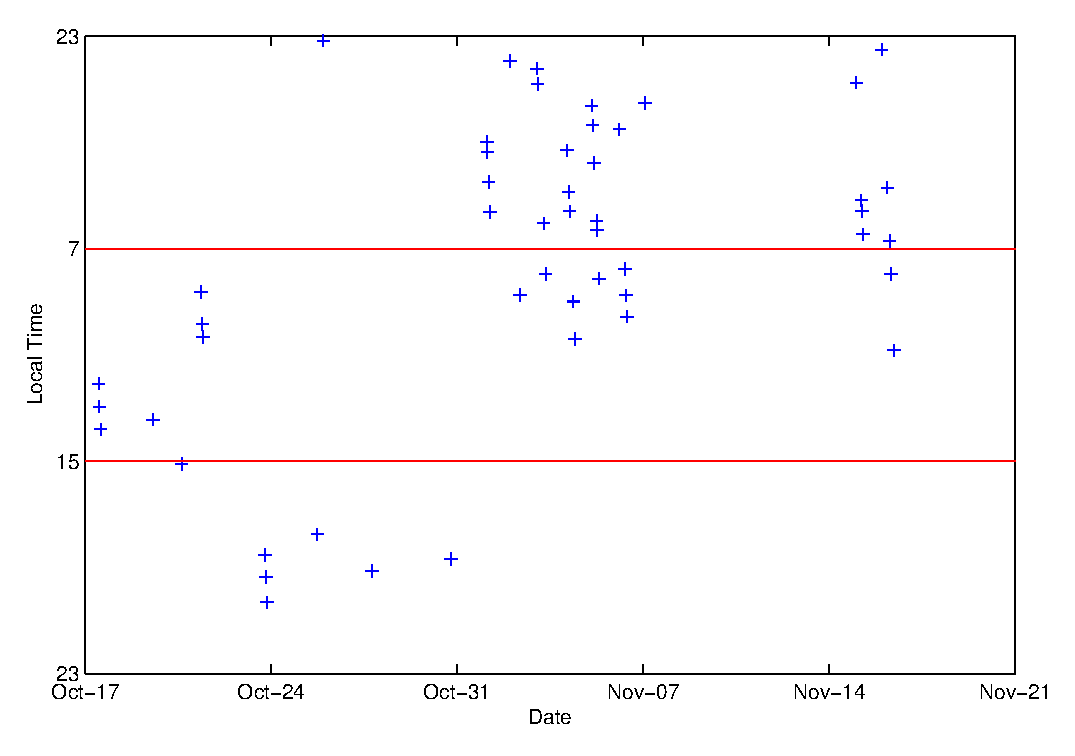
\includegraphics[width =8cm]{PlotTime2011_4.eps}
\\
\caption{Events(runs) clock time distribution - 2011}
\end{center}
\end{minipage}
\end{figure}


 
\end{document}